\sub{Developer Perspektive}
Die folgende Tabelle zeigt die Software-Anforderungen an eine offlinefähige Kontaktliste aus der EntwicklerInnenperspektive.
\begin{longtable}[c]{@{}
>{\columncolor[HTML]{CFFCC2}}l ll@{}}
\toprule
  \multicolumn{1}{p{0.15\textwidth}}{\cellcolor[HTML]{cffcc2}\textbf{ID}}
  & \multicolumn{1}{p{0.85\textwidth}}{\cellcolor[HTML]{cffcc2}\textbf{Anforderung aus Entwicklungsperspektive}}\\ \hline \noalign{\vskip 0.1cm}
\endfirsthead
%
\endhead
%
  \multicolumn{1}{l}{\cellcolor[HTML]{cffcc2}\textbf{User-Story 1}} &
  \multicolumn{1}{p{0.85\textwidth}}
  {Ich als EntwicklerIn möchte die Daten lokal und auf dem Server speichern, um deren Erreichbarkeit unabhängig vom Internetstatus zu gewährleisten.}\\
  \midrule
  %
  \multicolumn{1}{l}{\cellcolor[HTML]{cffcc2}\textbf{User-Story 2}} &
  \multicolumn{1}{p{0.85\textwidth}}
  {Ich als EntwicklerIn möchte ich nur die Adressbucheinträge oder deren Aktualisierungen laden, die sich nicht schon auf dem Endgerät befinden, um Datentraffic und Ladezeiten zu sparen.}\\
  \midrule
  %
  \multicolumn{1}{l}{\cellcolor[HTML]{cffcc2}\textbf{User-Story 3}} &
  \multicolumn{1}{p{0.85\textwidth}}
  {Ich als EntwicklerIn möchte ich jeden Eintrag identifizieren, um jedem Adressbucheintrag Operationen zuzuweisen und einzelne Kontakte zu finden.}\\
  \midrule
  %
  \multicolumn{1}{l}{\cellcolor[HTML]{cffcc2}\textbf{User-Story 4}} &
  \multicolumn{1}{p{0.85\textwidth}}
  {Ich als EntwicklerIn möchte ich jeden Eintrag versionieren, um zu wissen ob wann ein Eintrag bearbeitet wurde.}\\
  \midrule
  %
  \multicolumn{1}{l}{\cellcolor[HTML]{cffcc2}\textbf{User-Story 5}} &
  \multicolumn{1}{p{0.85\textwidth}}
  {Ich als EntwicklerIn möchte dass alle von NutzerInnen vorgenommenen Änderungen beim System ankommen und keine Daten verloren gehen.}\\
  \midrule
  %
  \multicolumn{1}{l}{\cellcolor[HTML]{cffcc2}\textbf{User-Story 6}} &
  \multicolumn{1}{p{0.85\textwidth}}
  {Ich als EntwicklerIn möchte auftretende Konflikte effizient speichern, um mit ihnen umgehen können. \todo{Mit ihnen umgehen heißt: selbstständig oder von User lösen, zum konfliktfreien Zustand gelangen}}\\
  \midrule
  %
  \multicolumn{1}{l}{\cellcolor[HTML]{cffcc2}\textbf{User-Story 7}} &
  \multicolumn{1}{p{0.85\textwidth}}
  {Ich als EntwicklerIn möchte eine Technologie verwenden die leicht zu verstehen und implemenieren ist, um den Arbeitsaufwand gering zu halten.}\\
  \midrule
  %
  \multicolumn{1}{l}{\cellcolor[HTML]{cffcc2}\textbf{User-Story 6}} &
  \multicolumn{1}{p{0.85\textwidth}}
  {Ich als EntwicklerIn möchte sauberen und verständlichen Code schreiben, um die Les-- und Wartbarkeit zu erhöhen.}\\
  % end
  \bottomrule \cellcolor[HTML]{FFFFFF}
  \vspace{0.1cm}\\
  \noalign{\hspace{0.0525\textwidth}\grayRule}
  \caption{Anforderungen aus Entwicklungsperspektive}
  \label{tab:dev}\\
\end{longtable}
%
% Das in Abbildung \ref{fig:uc} gezeigte Use-Case-Diagramm veranschaulicht die in der obigen Tabelle \ref{tab:dev} aufgeführten Anwendungsfälle.
% \begin{figure}[H]
%     \centering
%     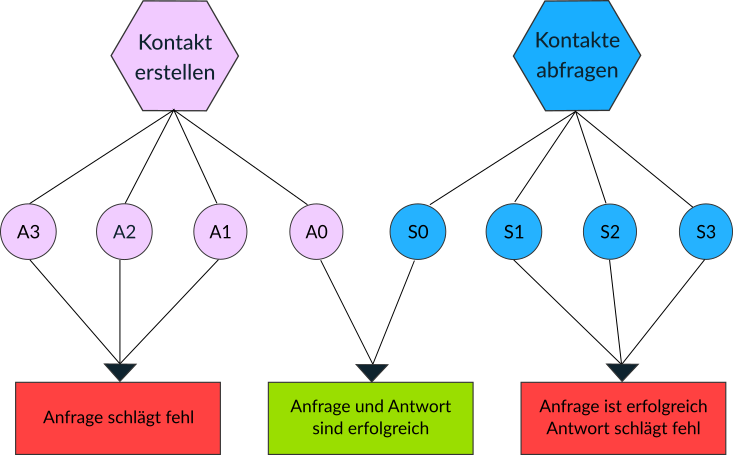
\includegraphics[width=0.4\textwidth]{Szenarien}
%     \grayRule
%     \caption[Use-Case Diagramm]{Platzhalter für US-Diagramm}
%     \label{fig:uc}
% \end{figure}